%\section {Random methods}

%
%  random methods
%

\begin{frame} {Random methods}
  \begin{itemize}
  \item In the early 1990's, random methods started being developed
    \pause
  \item Principle
    \begin{itemize}
    \item shoot random configurations
      \pause
    \item test whether they are in collision
      \pause
    \item build a graph (roadmap)  the nodes of which are free configurations
      \pause
    \item  and the edges of which are collision-free linear interpolations
    \end{itemize}
  \end{itemize}
\end{frame}

%
%  La méthode du réseau aléatoire
%

\begin{frame} {Probabilistic roadmap (PRM) 1994}
\centerline {
  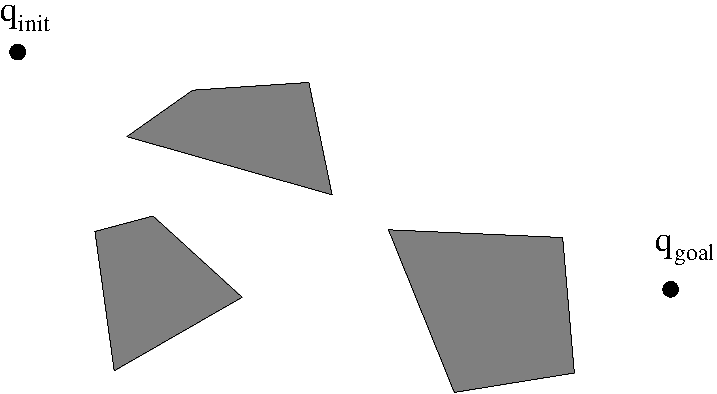
\includegraphics[width=.8\linewidth]{figures/PRM1.pdf}
}
\end{frame}

\begin{frame} {Probabilistic roadmap (PRM) 1994}
\centerline {
  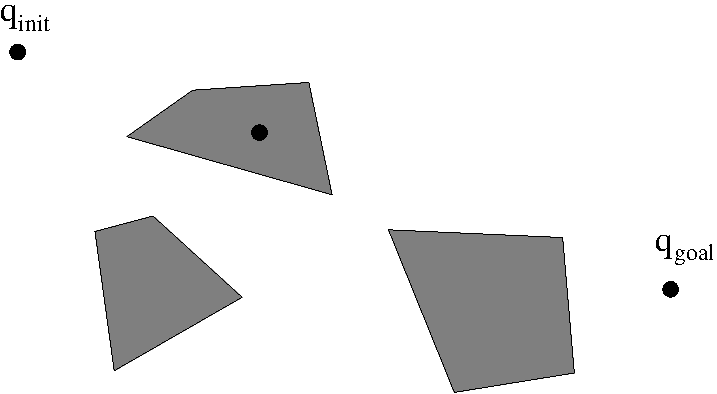
\includegraphics[width=.8\linewidth]{figures/PRM2.pdf}
}
\end{frame}

\begin{frame} {Probabilistic roadmap (PRM) 1994}
\centerline {
  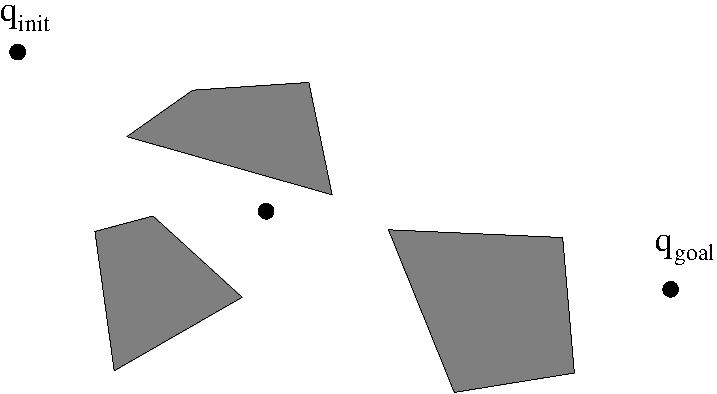
\includegraphics[width=.8\linewidth]{figures/PRM3.pdf}
}
\end{frame}

\begin{frame} {Probabilistic roadmap (PRM) 1994}
\centerline {
  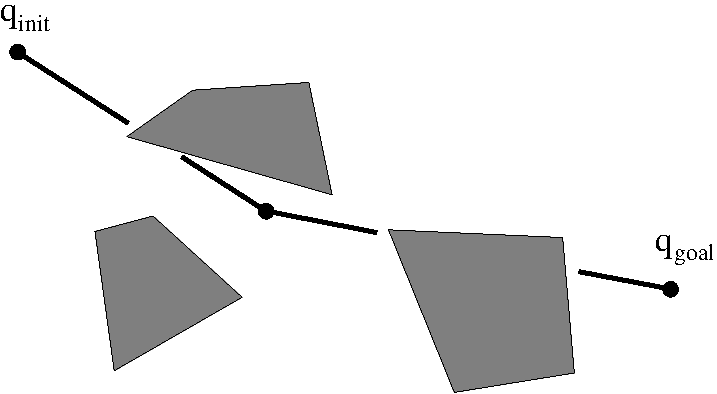
\includegraphics[width=.8\linewidth]{figures/PRM4.pdf}
}
\end{frame}

\begin{frame} {Probabilistic roadmap (PRM) 1994}
\centerline {
  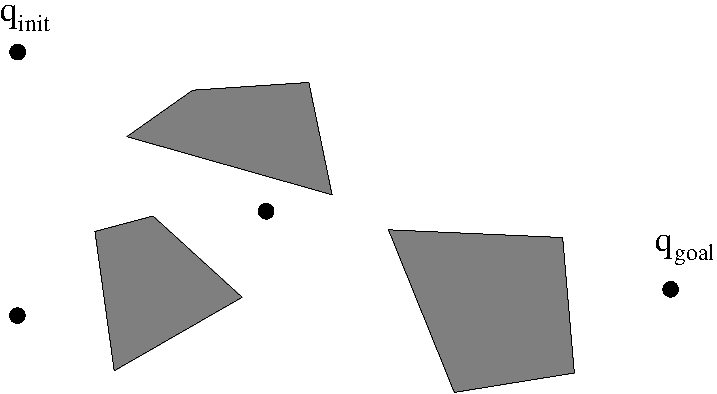
\includegraphics[width=.8\linewidth]{figures/PRM5.pdf}
}
\end{frame}

\begin{frame} {Probabilistic roadmap (PRM) 1994}
\centerline {
  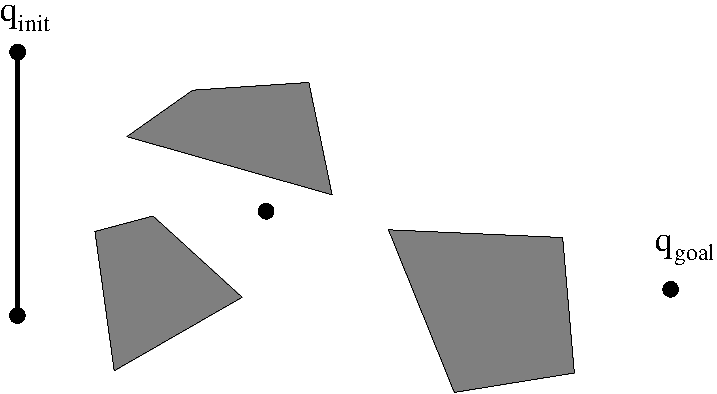
\includegraphics[width=.8\linewidth]{figures/PRM6.pdf}
}
\end{frame}

\begin{frame} {Probabilistic roadmap (PRM) 1994}
\centerline {
  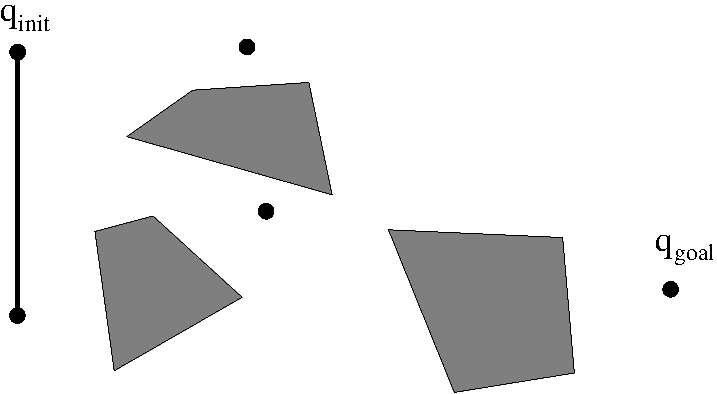
\includegraphics[width=.8\linewidth]{figures/PRM7.pdf}
}
\end{frame}

\begin{frame} {Probabilistic roadmap (PRM) 1994}
\centerline {
  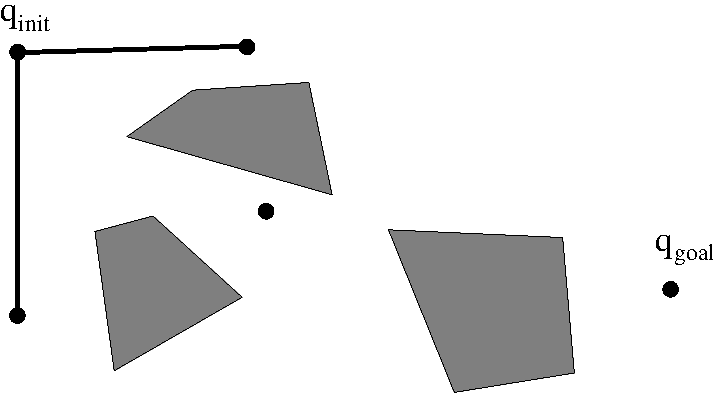
\includegraphics[width=.8\linewidth]{figures/PRM8.pdf}
}
\end{frame}

\begin{frame} {Probabilistic roadmap (PRM) 1994}
\centerline {
  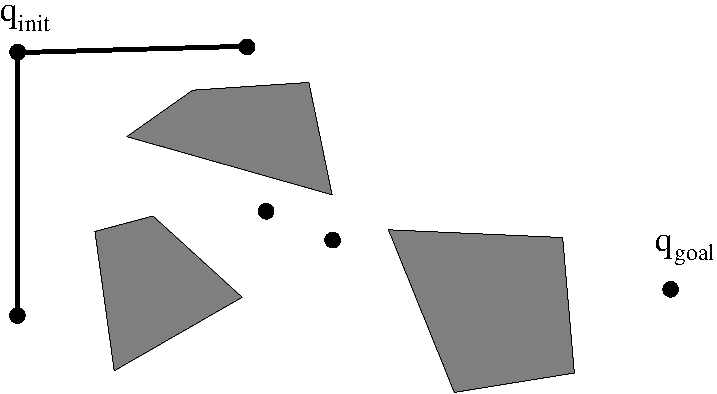
\includegraphics[width=.8\linewidth]{figures/PRM9.pdf}
}
\end{frame}

\begin{frame} {Probabilistic roadmap (PRM) 1994}
\centerline {
  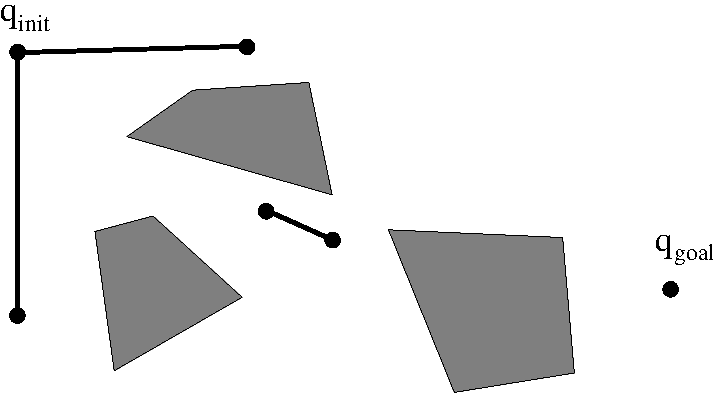
\includegraphics[width=.8\linewidth]{figures/PRM10.pdf}
}
\end{frame}

\begin{frame} {Probabilistic roadmap (PRM) 1994}
\centerline {
  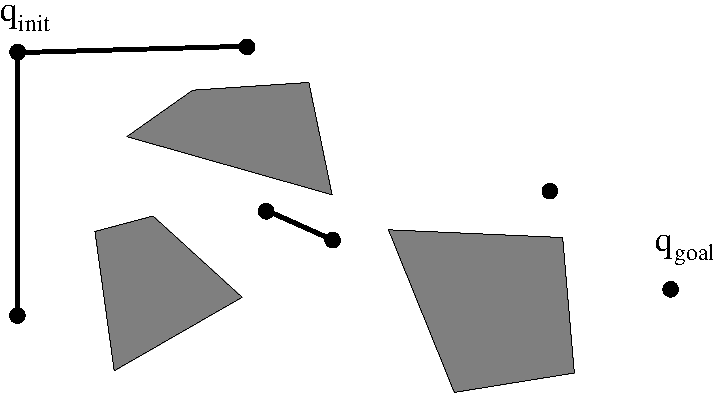
\includegraphics[width=.8\linewidth]{figures/PRM11.pdf}
}
\end{frame}

\begin{frame} {Probabilistic roadmap (PRM) 1994}
\centerline {
  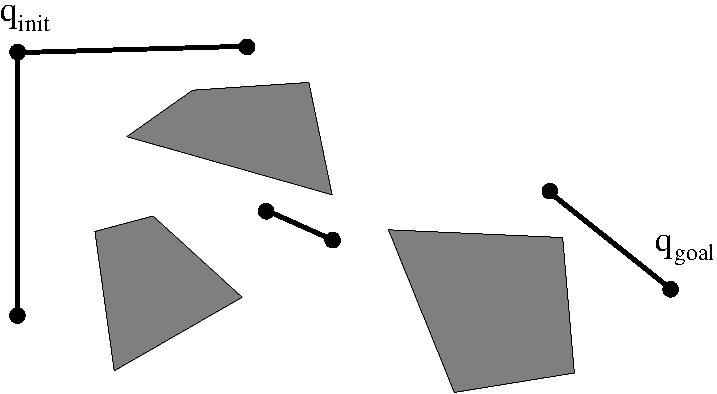
\includegraphics[width=.8\linewidth]{figures/PRM12.pdf}
}
\end{frame}

\begin{frame} {Probabilistic roadmap (PRM) 1994}
\centerline {
  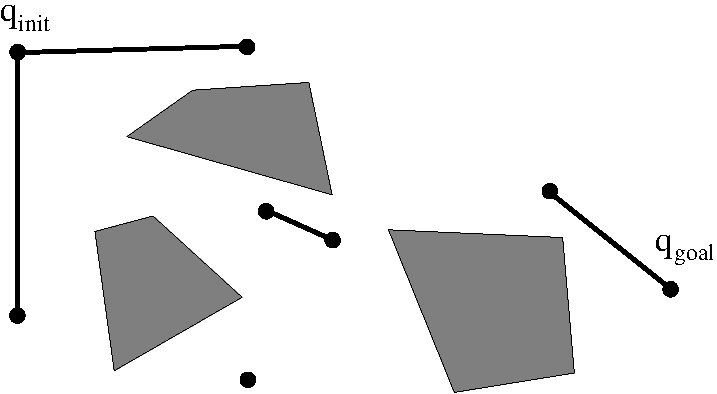
\includegraphics[width=.8\linewidth]{figures/PRM13.pdf}
}
\end{frame}

\begin{frame} {Probabilistic roadmap (PRM) 1994}
\centerline {
  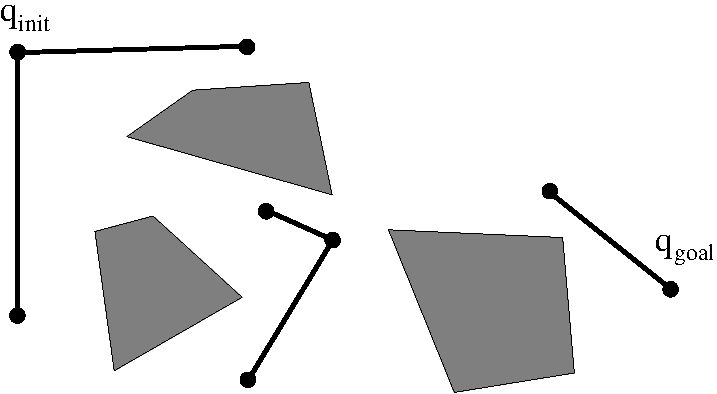
\includegraphics[width=.8\linewidth]{figures/PRM14.pdf}
}
\end{frame}

\begin{frame} {Probabilistic roadmap (PRM) 1994}
\centerline {
  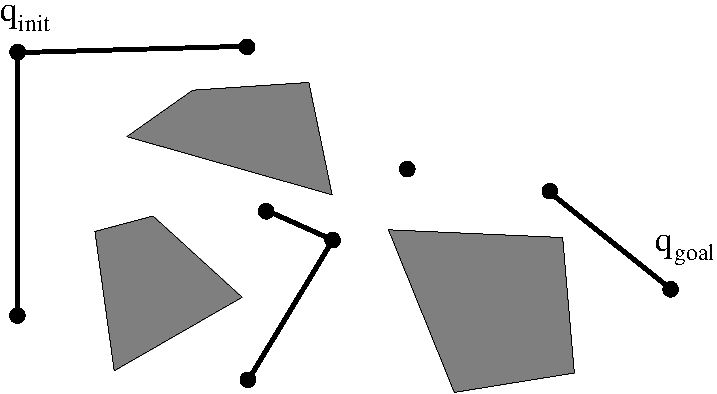
\includegraphics[width=.8\linewidth]{figures/PRM15.pdf}
}
\end{frame}

\begin{frame} {Probabilistic roadmap (PRM) 1994}
\centerline {
  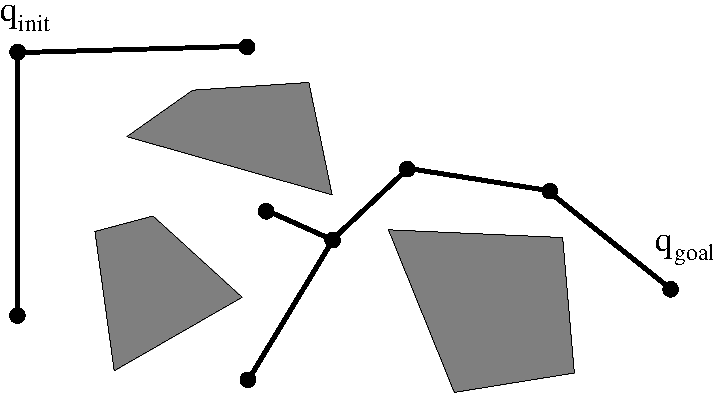
\includegraphics[width=.8\linewidth]{figures/PRM16.pdf}
}
\end{frame}

\begin{frame} {Probabilistic roadmap (PRM) 1994}
\centerline {
  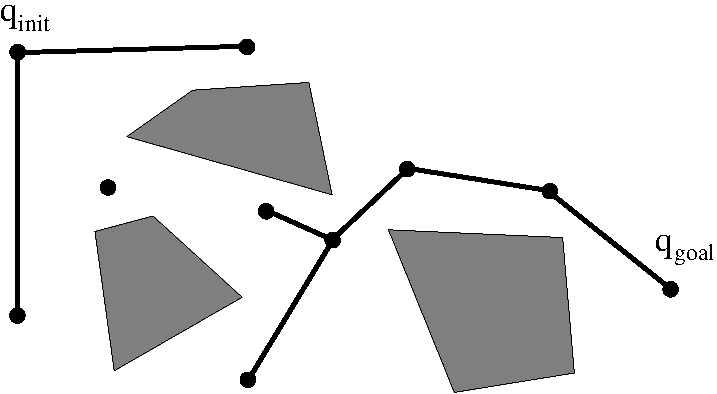
\includegraphics[width=.8\linewidth]{figures/PRM17.pdf}
}
\end{frame}

\begin{frame} {Probabilistic roadmap (PRM) 1994}
\centerline {
  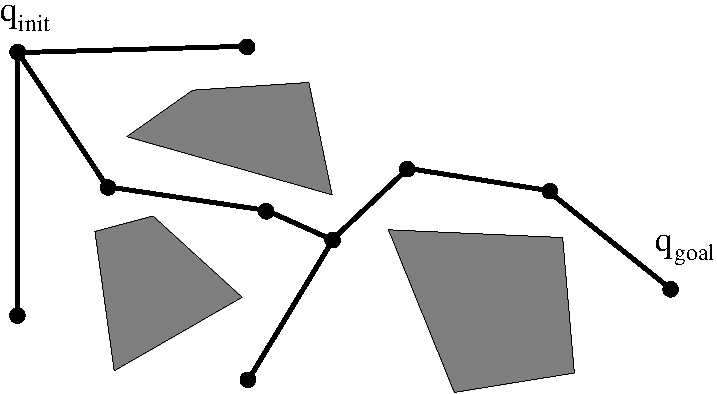
\includegraphics[width=.8\linewidth]{figures/PRM18.pdf}
}
\end{frame}

\begin{frame} {Probabilistic roadmap (PRM)}
  \begin{itemize}
  \item A lot of useless nodes are created,
    \begin{itemize}
    \item this increases the cost to connect new nodes to the existing roadmap
    \end{itemize}
  \item Improvement: visibility-based PRM
    \begin{itemize}
    \item Only \textit{interesting} nodes are kept.
    \end{itemize}
  \end{itemize}
\end{frame}


%
%  Visibility-based probabilistic roadmap
%
\begin{frame} {Visibility-based probabilistic roadmap (Visi-PRM) 1999}
\centerline {
  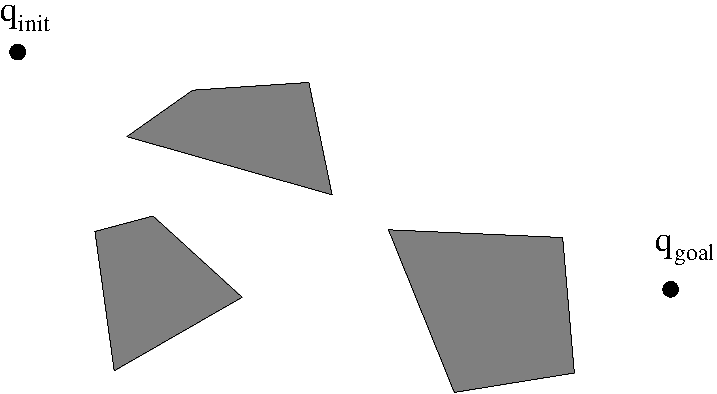
\includegraphics[width=.8\linewidth]{figures/VPRM1.pdf}
}
\end{frame}

\begin{frame} {Visibility-based probabilistic roadmap (Visi-PRM) 1999}
\centerline {
  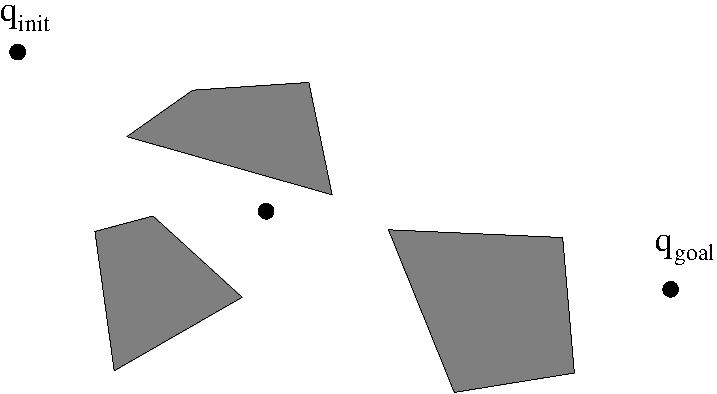
\includegraphics[width=.8\linewidth]{figures/VPRM2.pdf}
}
\end{frame}

\begin{frame} {Visibility-based probabilistic roadmap (Visi-PRM) 1999}
\centerline {
  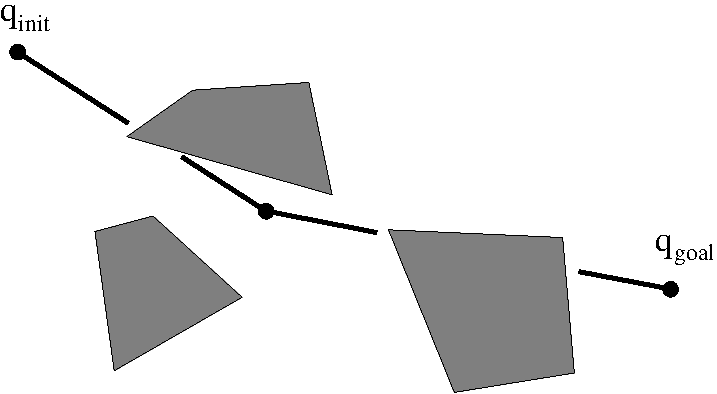
\includegraphics[width=.8\linewidth]{figures/VPRM3.pdf}
}
\end{frame}

\begin{frame} {Visibility-based probabilistic roadmap (Visi-PRM) 1999}
\centerline {
  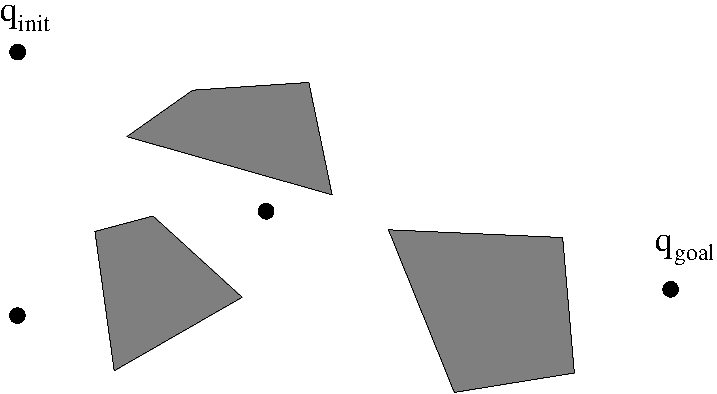
\includegraphics[width=.8\linewidth]{figures/VPRM4.pdf}
}
\end{frame}

\begin{frame} {Visibility-based probabilistic roadmap (Visi-PRM) 1999}
\centerline {
  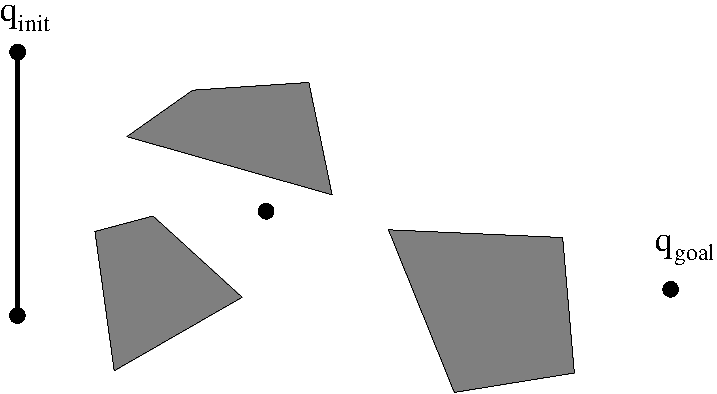
\includegraphics[width=.8\linewidth]{figures/VPRM5.pdf}
}
\end{frame}

\begin{frame} {Visibility-based probabilistic roadmap (Visi-PRM) 1999}
\centerline {
  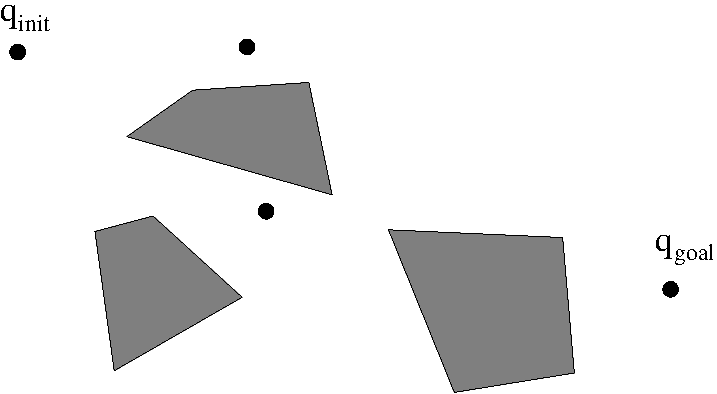
\includegraphics[width=.8\linewidth]{figures/VPRM6.pdf}
}
\end{frame}

\begin{frame} {Visibility-based probabilistic roadmap (Visi-PRM) 1999}
\centerline {
  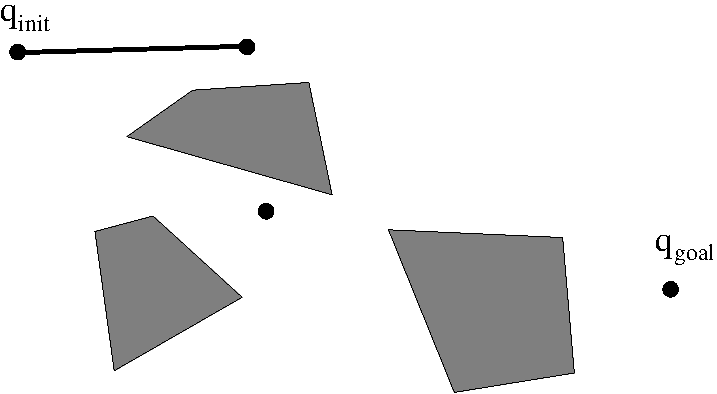
\includegraphics[width=.8\linewidth]{figures/VPRM7.pdf}
}
\end{frame}

\begin{frame} {Visibility-based probabilistic roadmap (Visi-PRM) 1999}
\centerline {
  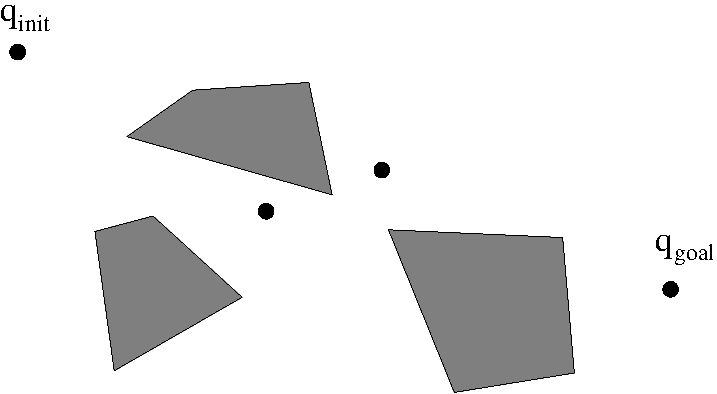
\includegraphics[width=.8\linewidth]{figures/VPRM8.pdf}
}
\end{frame}

\begin{frame} {Visibility-based probabilistic roadmap (Visi-PRM) 1999}
\centerline {
  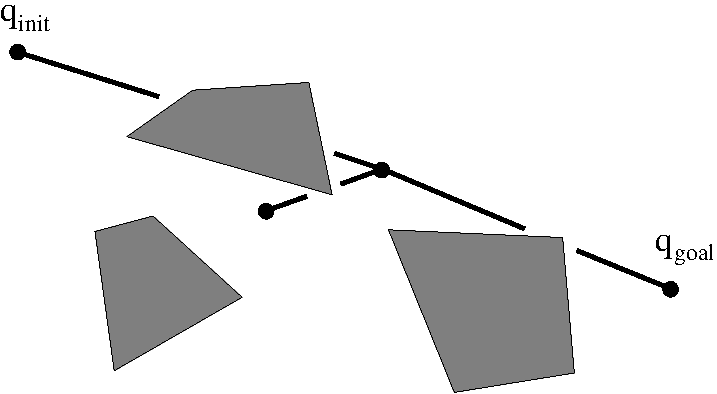
\includegraphics[width=.8\linewidth]{figures/VPRM9.pdf}
}
\end{frame}

\begin{frame} {Visibility-based probabilistic roadmap (Visi-PRM) 1999}
\centerline {
  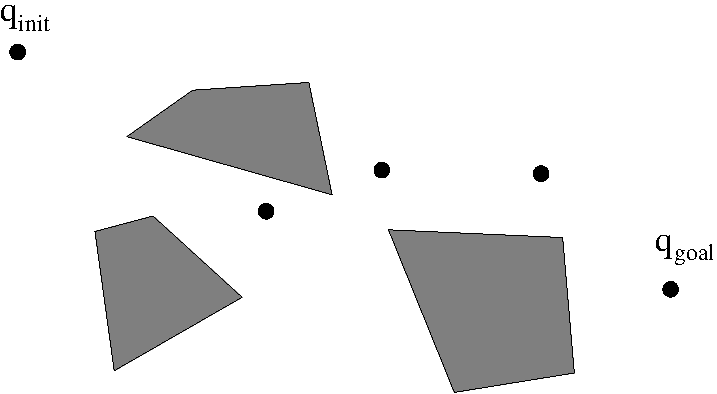
\includegraphics[width=.8\linewidth]{figures/VPRM10.pdf}
}
\end{frame}

\begin{frame} {Visibility-based probabilistic roadmap (Visi-PRM) 1999}
\centerline {
  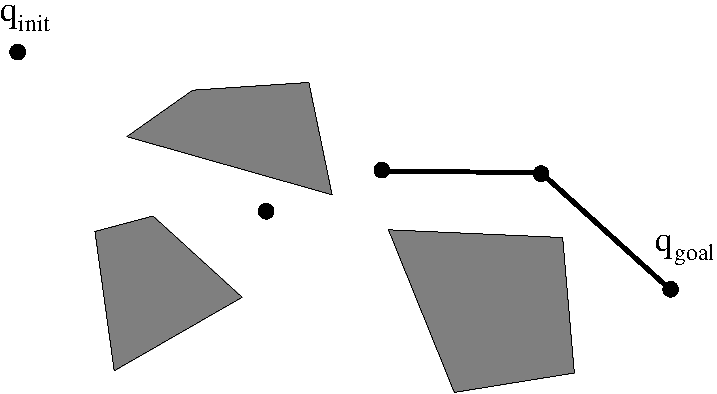
\includegraphics[width=.8\linewidth]{figures/VPRM11.pdf}
}
\end{frame}

\begin{frame} {Visibility-based probabilistic roadmap (Visi-PRM) 1999}
\centerline {
  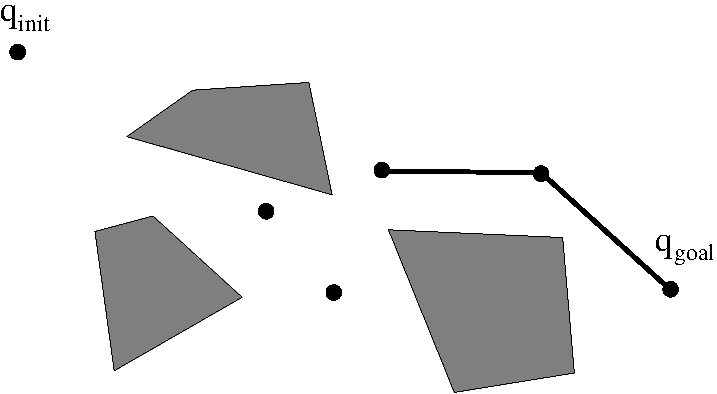
\includegraphics[width=.8\linewidth]{figures/VPRM12.pdf}
}
\end{frame}

\begin{frame} {Visibility-based probabilistic roadmap (Visi-PRM) 1999}
\centerline {
  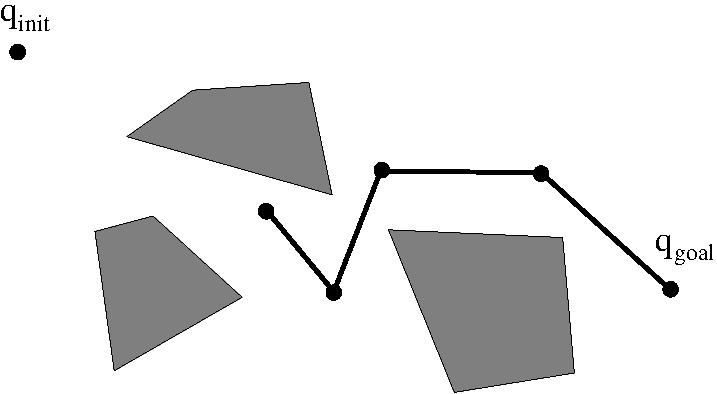
\includegraphics[width=.8\linewidth]{figures/VPRM13.pdf}
}
\end{frame}

\begin{frame} {Visibility-based probabilistic roadmap (Visi-PRM) 1999}
\centerline {
  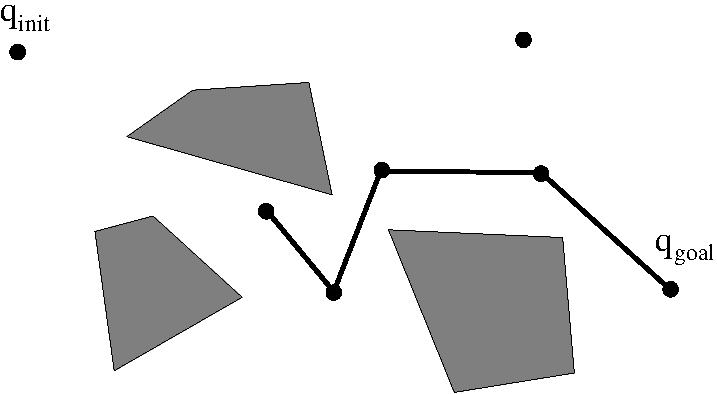
\includegraphics[width=.8\linewidth]{figures/VPRM14.pdf}
}
\end{frame}

\begin{frame} {Visibility-based probabilistic roadmap (Visi-PRM) 1999}
\centerline {
  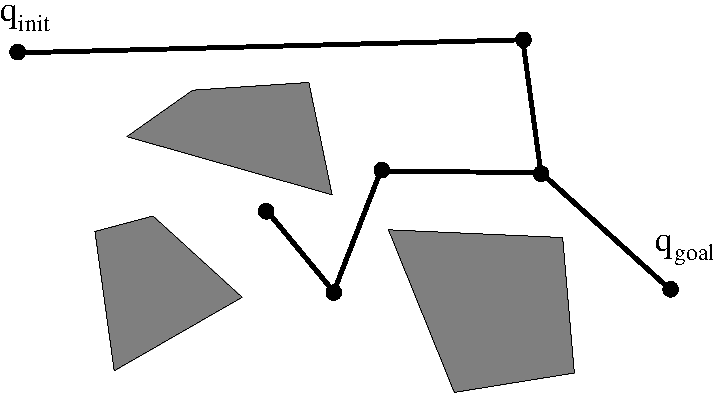
\includegraphics[width=.8\linewidth]{figures/VPRM15.pdf}
}
\end{frame}

%
%  La méthode des arbres aléatoires d'exploration rapide.
%

\begin{frame} {Rapidly exploring Random Tree (RRT) 2000}
\centerline {
  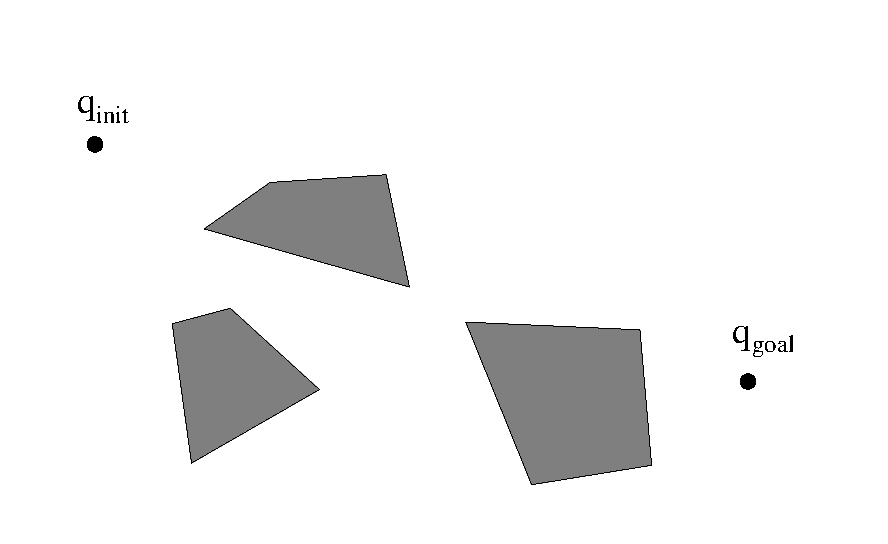
\includegraphics[width=.8\linewidth]{figures/RRT1.pdf}
}
\end{frame}

\begin{frame} {Rapidly exploring Random Tree (RRT) 2000}
\centerline {
  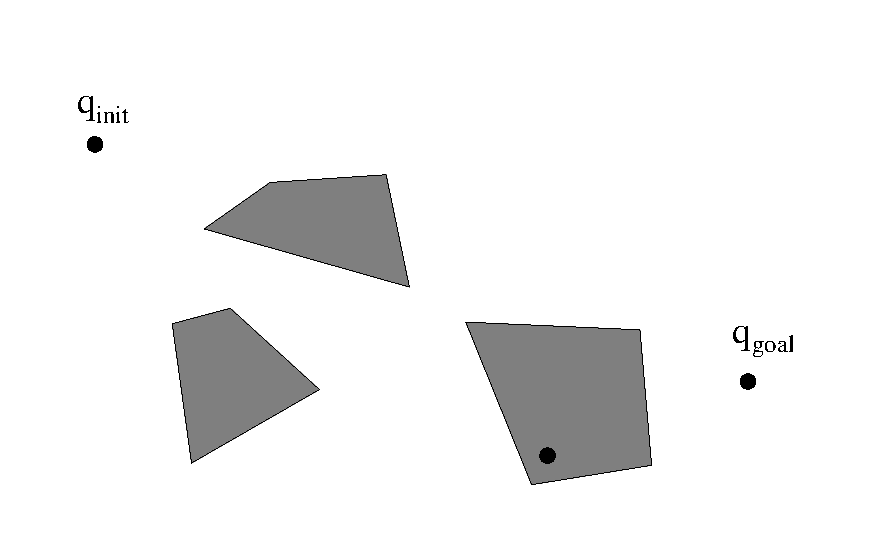
\includegraphics[width=.8\linewidth]{figures/RRT2.pdf}
}
\end{frame}

\begin{frame} {Rapidly exploring Random Tree (RRT) 2000}
\centerline {
  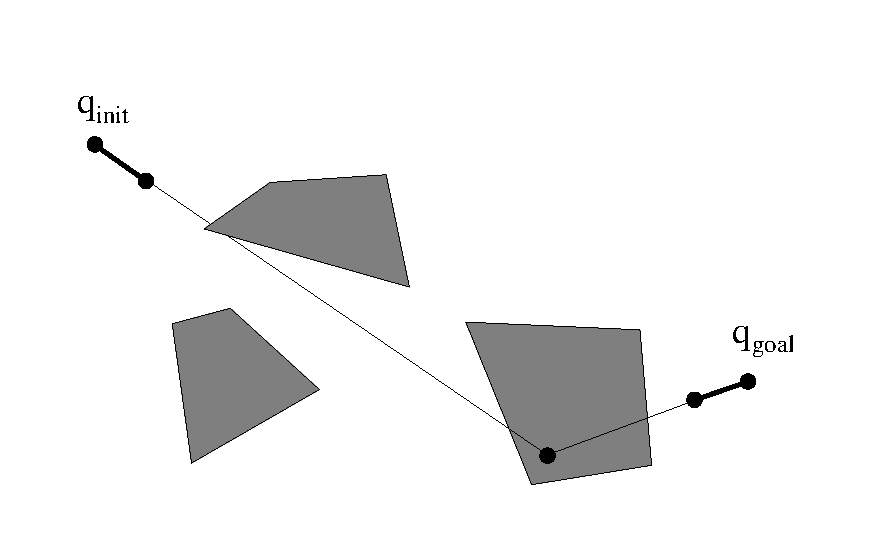
\includegraphics[width=.8\linewidth]{figures/RRT3.pdf}
}
\end{frame}

\begin{frame} {Rapidly exploring Random Tree (RRT) 2000}
\centerline {
  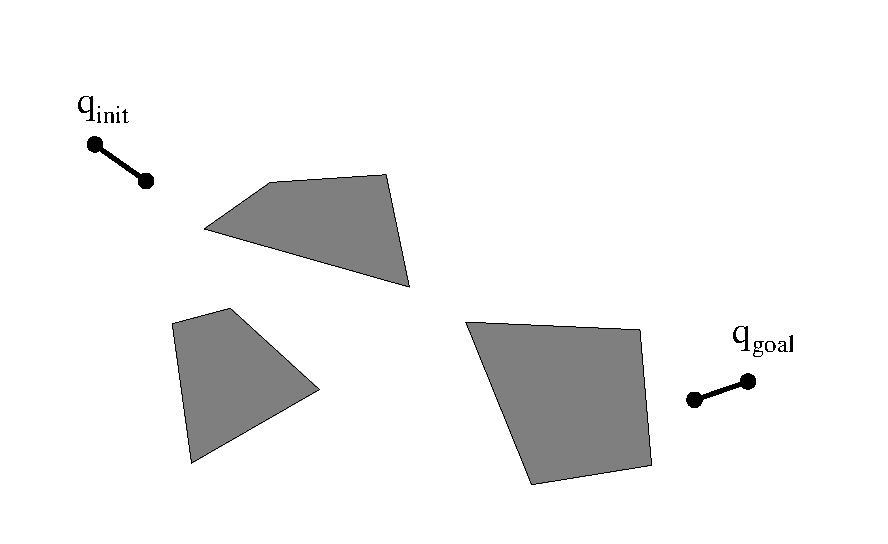
\includegraphics[width=.8\linewidth]{figures/RRT4.pdf}
}
\end{frame}

\begin{frame} {Rapidly exploring Random Tree (RRT) 2000}
\centerline {
  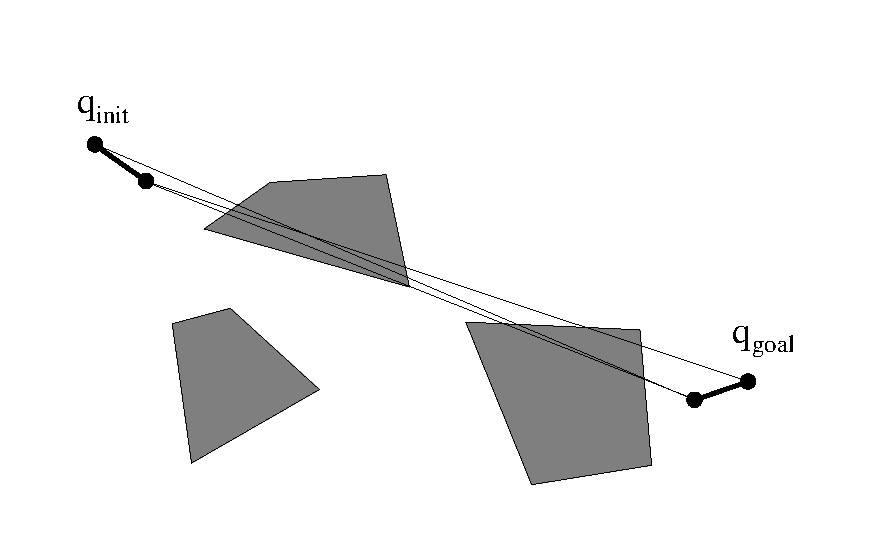
\includegraphics[width=.8\linewidth]{figures/RRT5.pdf}
}
\end{frame}

\begin{frame} {Rapidly exploring Random Tree (RRT) 2000}
\centerline {
  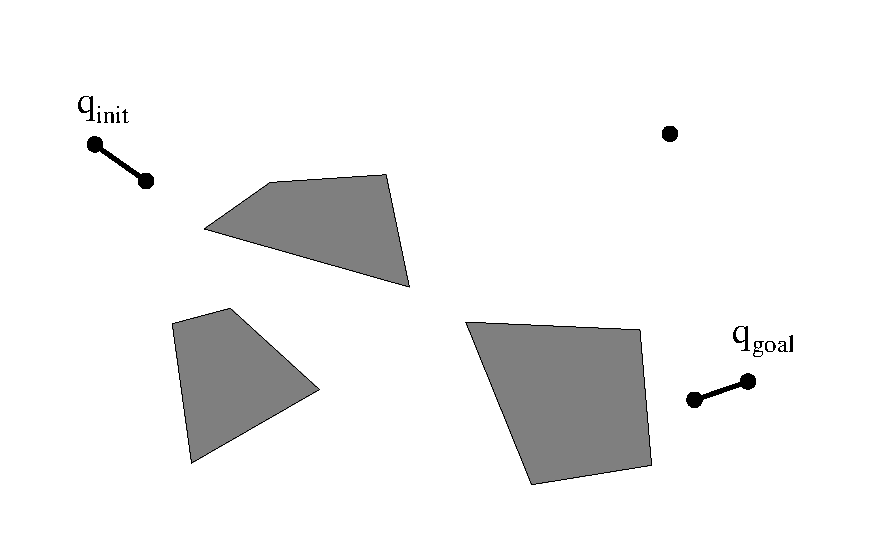
\includegraphics[width=.8\linewidth]{figures/RRT6.pdf}
}
\end{frame}

\begin{frame} {Rapidly exploring Random Tree (RRT) 2000}
\centerline {
  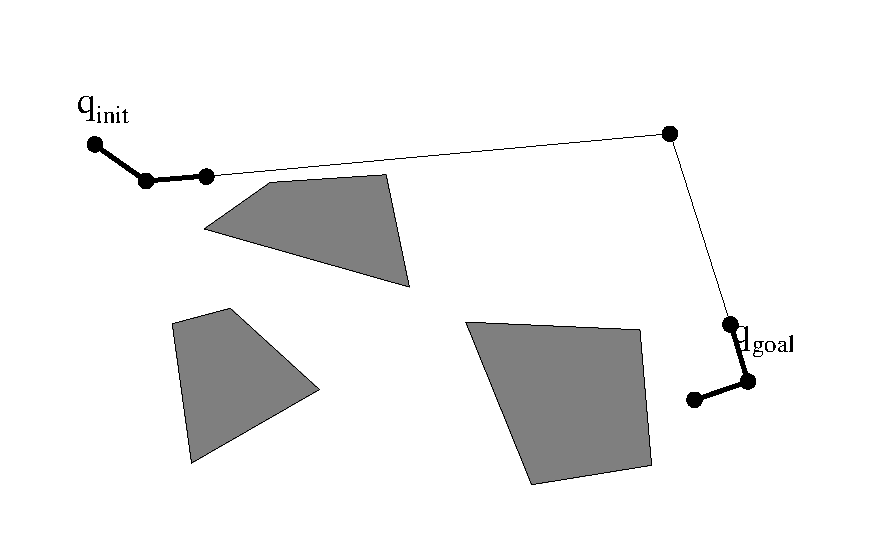
\includegraphics[width=.8\linewidth]{figures/RRT7.pdf}
}
\end{frame}

\begin{frame} {Rapidly exploring Random Tree (RRT) 2000}
\centerline {
  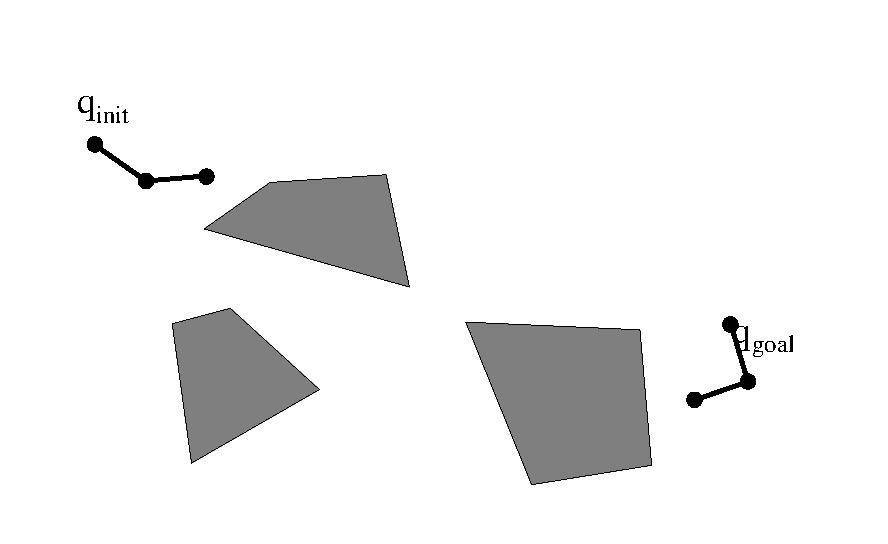
\includegraphics[width=.8\linewidth]{figures/RRT8.pdf}
}
\end{frame}

\begin{frame} {Rapidly exploring Random Tree (RRT) 2000}
\centerline {
  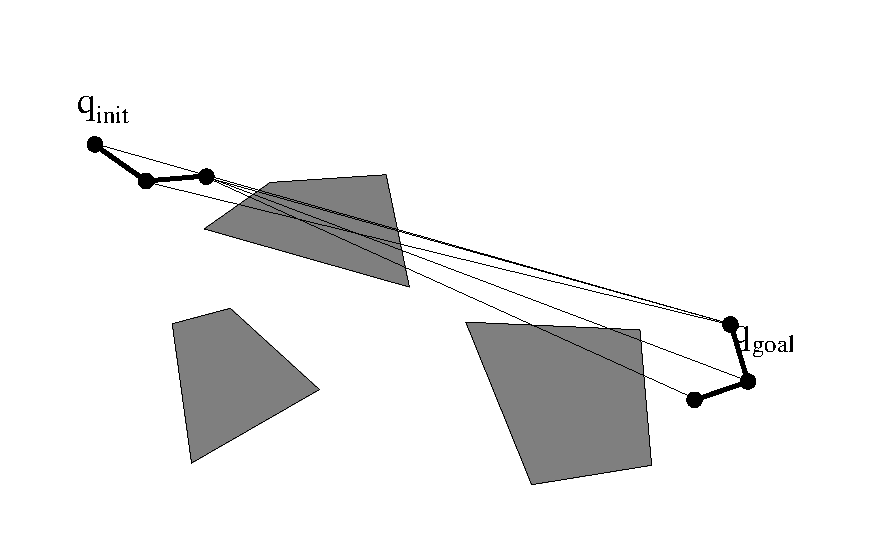
\includegraphics[width=.8\linewidth]{figures/RRT9.pdf}
}
\end{frame}

\begin{frame} {Rapidly exploring Random Tree (RRT) 2000}
\centerline {
  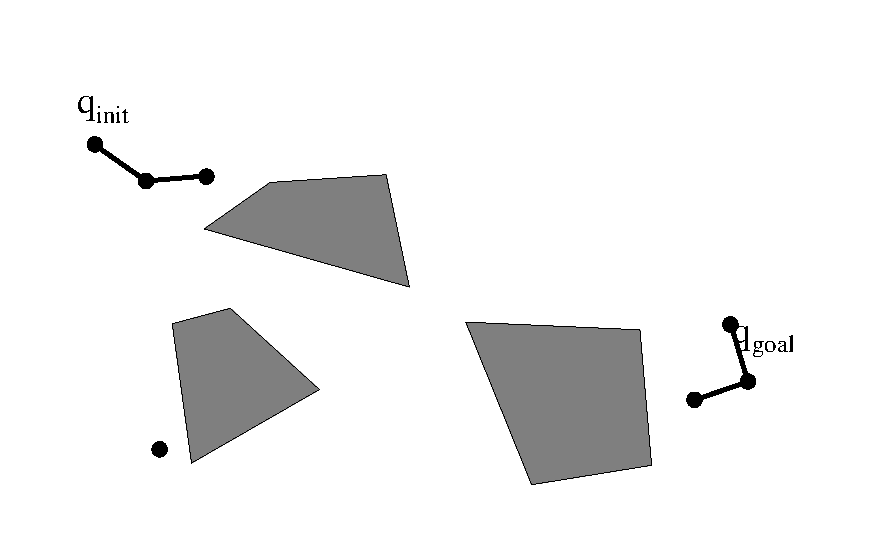
\includegraphics[width=.8\linewidth]{figures/RRT10.pdf}
}
\end{frame}

\begin{frame} {Rapidly exploring Random Tree (RRT) 2000}
\centerline {
  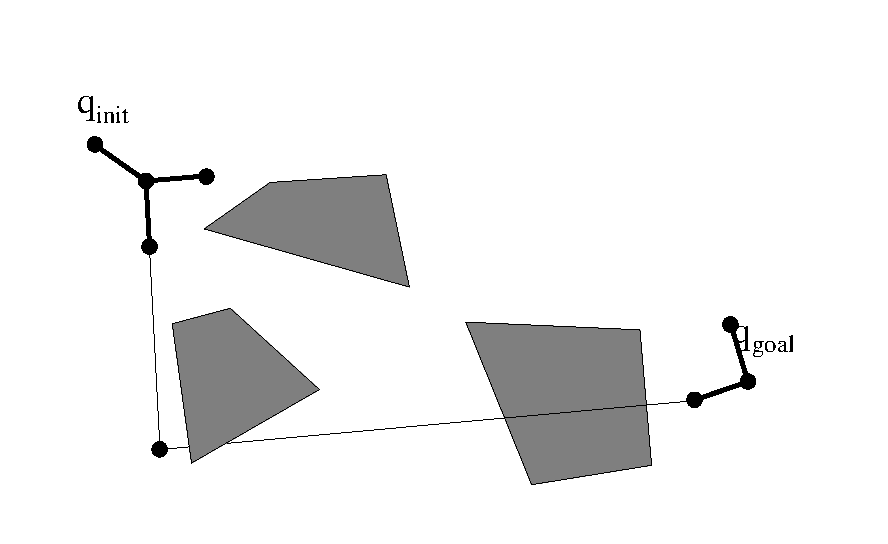
\includegraphics[width=.8\linewidth]{figures/RRT11.pdf}
}
\end{frame}

\begin{frame} {Rapidly exploring Random Tree (RRT) 2000}
\centerline {
  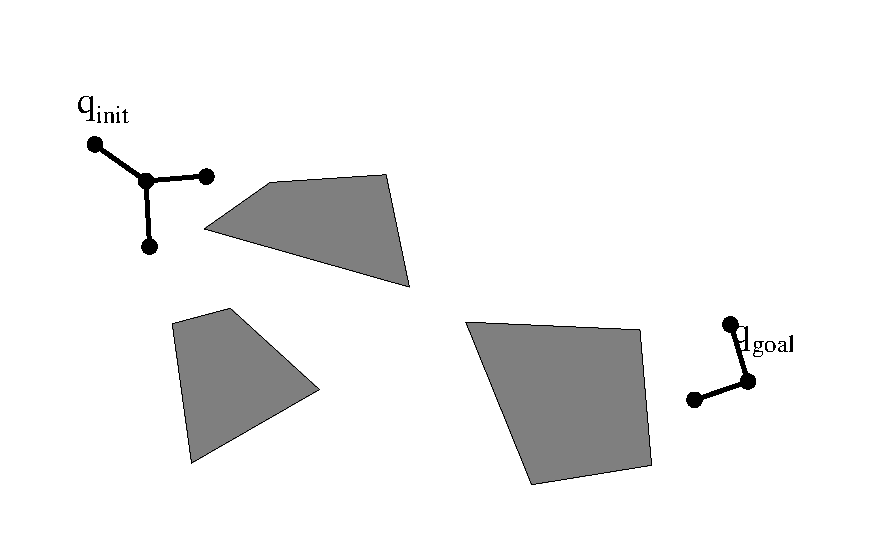
\includegraphics[width=.8\linewidth]{figures/RRT12.pdf}
}
\end{frame}

\begin{frame} {Rapidly exploring Random Tree (RRT) 2000}
\centerline {
  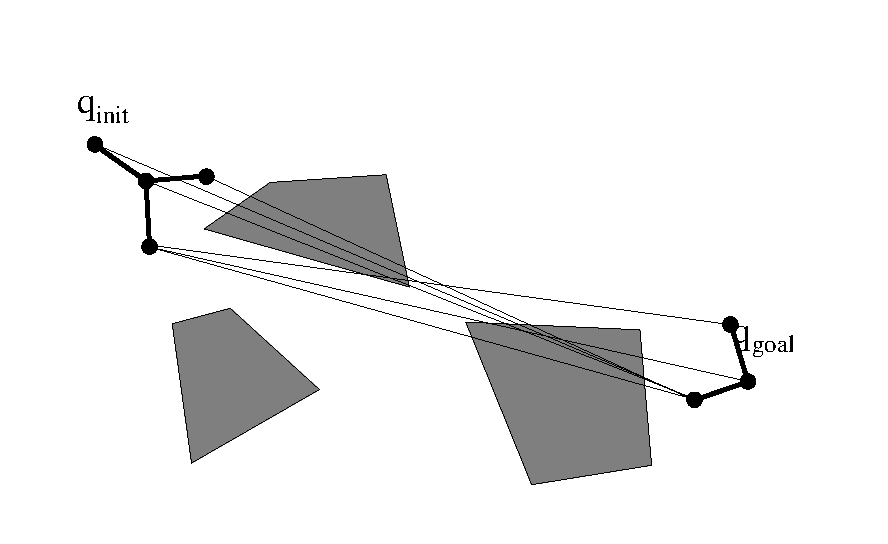
\includegraphics[width=.8\linewidth]{figures/RRT13.pdf}
}
\end{frame}

\begin{frame} {Rapidly exploring Random Tree (RRT) 2000}
\centerline {
  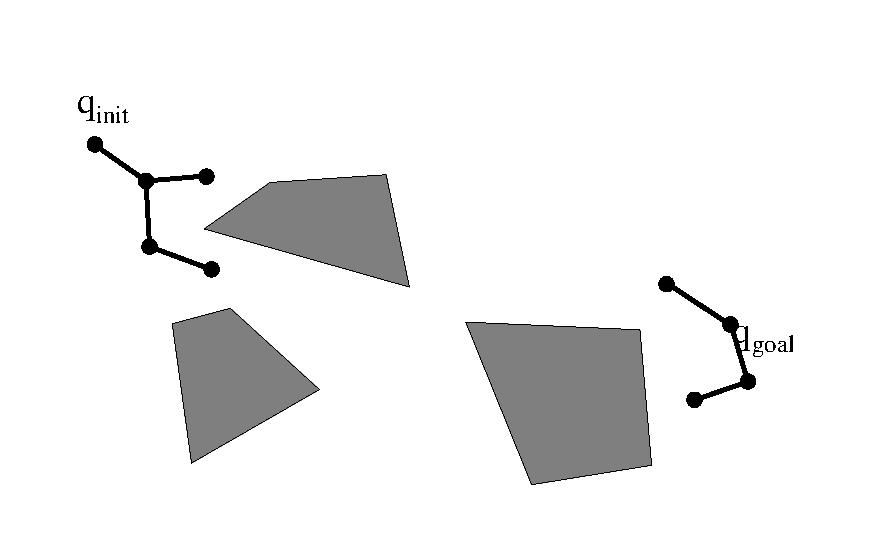
\includegraphics[width=.8\linewidth]{figures/RRT14.pdf}
}
\end{frame}

\begin{frame} {Rapidly exploring Random Tree (RRT) 2000}
\centerline {
  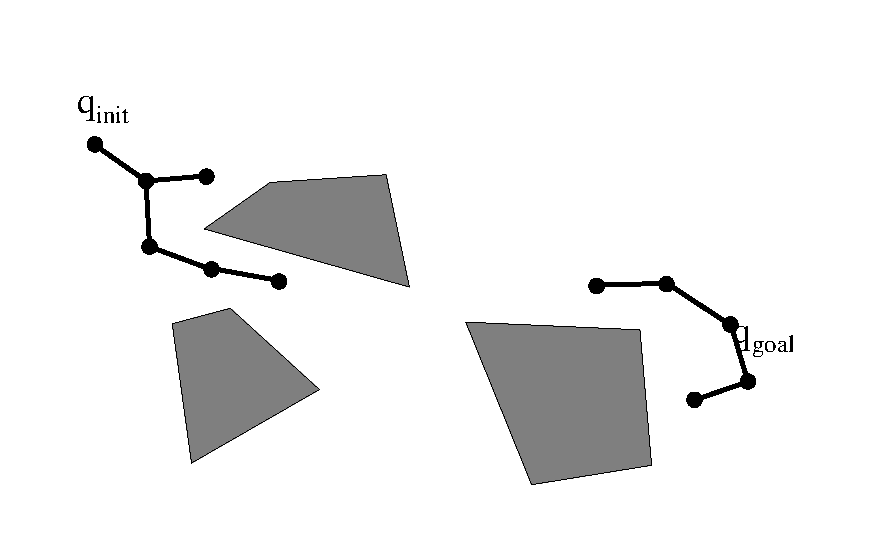
\includegraphics[width=.8\linewidth]{figures/RRT15.pdf}
}
\end{frame}

\begin{frame} {Rapidly exploring Random Tree (RRT) 2000}
\centerline {
  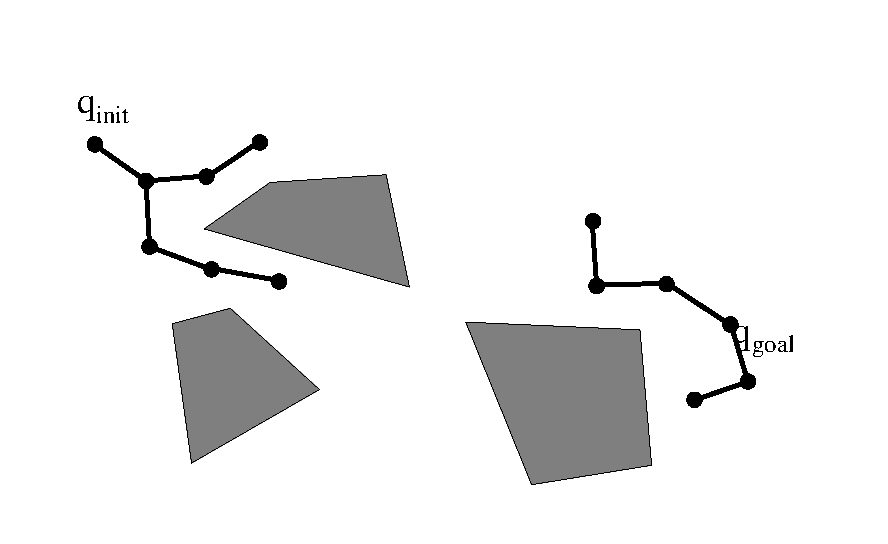
\includegraphics[width=.8\linewidth]{figures/RRT16.pdf}
}
\end{frame}

\begin{frame} {Rapidly exploring Random Tree (RRT) 2000}
\centerline {
  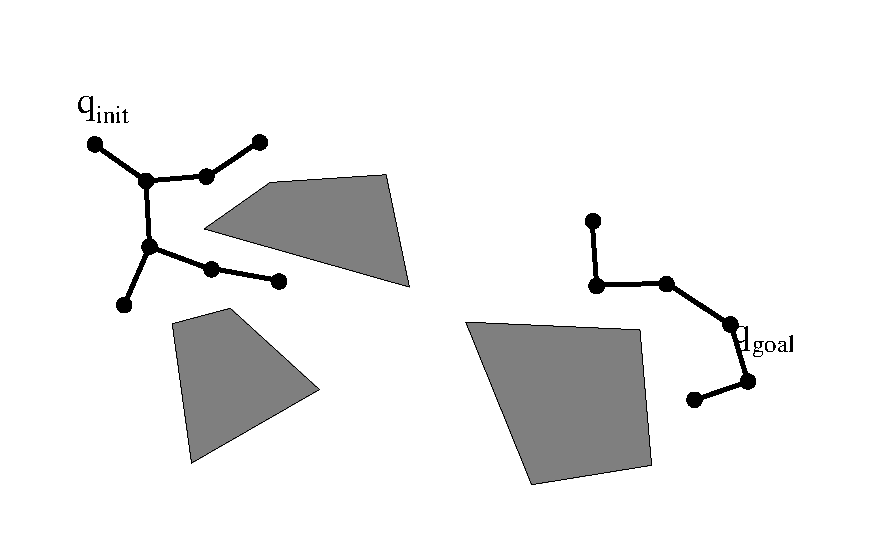
\includegraphics[width=.8\linewidth]{figures/RRT17.pdf}
}
\end{frame}

\begin{frame} {Rapidly exploring Random Tree (RRT) 2000}
\centerline {
  \includegraphics[width=.8\linewidth]{figures/RRT18.pdf}
}
\end{frame}

\begin{frame} {Rapidly exploring Random Tree (RRT) 2000}
\centerline {
  \includegraphics[width=.8\linewidth]{figures/RRT19.pdf}
}
\end{frame}

\begin{frame} {Rapidly exploring Random Tree (RRT) 2000}
\centerline {
  \includegraphics[width=.8\linewidth]{figures/RRT20.pdf}
}
\end{frame}

%
% random methods
%

\begin{frame} {Random methods}
  \begin{itemize}
  \item Pros:
    \begin{itemize}
    \item no explicit computation of the free configuration space,
    \item easy to implement,
    \item robust.
    \end{itemize}
    \pause
  \item Cons:
    \begin{itemize}
    \item no completeness property, only probabilistic completeness,
    \item difficult to find narrow passages.
    \end{itemize}
    \pause
  \item Requested operators~:
    \begin{itemize}
    \item Collision tests
      \begin{itemize}
      \item for configurations (static),
      \item for paths (dynamic)
      \end{itemize}
    \end{itemize}
  \end{itemize}
\end{frame}
